\documentclass[openany]{article}
%\usepackage[english]{babel}
\usepackage[spanish]{babel}
\usepackage{commands}
\usepackage{xcolor}

\usepackage{lipsum}
\usepackage{algorithm}
\usepackage{algpseudocode}
\usepackage{float}
\usepackage{svg}
\pagestyle{fancy}
\fancyhf{}
\lhead{}
\rhead{\leftmark}
\cfoot{\thepage}

\setlength{\parskip}{4mm}

\addbibresource{references.bib}

% Cambiar "Algorithm" por "Algoritmo" en el título del algoritmo
\makeatletter
\renewcommand{\ALG@name}{Algoritmo}
\makeatother

\begin{document}

\counterwithout{equation}{section}

\thispagestyle{empty}    

\begin{titlepage}
\begin{figure}[th]
\begin{flushleft}
    \includegraphics[width=7cm]{Figures/image1.png}
\end{flushleft}
\end{figure}
 \vspace{1cm}

{\flushleft \LARGE \bfseries TRABAJO DE FIN DE MÁSTER\par}\vspace{2cm}

% Thesis title
{\flushright \LARGE \bfseries Optimización de la carga manual de contenedores con paquetes heterogéneos  \par}\vspace{2cm}

{\flushleft \LARGE \bfseries Jose Gustavo Quilca Vilcapoma \par}\vspace{1.5cm}

{\flushleft \bfseries Máster Universitario en Estadística Computacional y Ciencia de Datos para la Toma de Decisiones\par}\vspace{0.cm}
{\flushleft \bfseries (Specialization/Pathway in XXXX)\par}\vspace{0.cm}
{\flushleft \bfseries Instituto de investigación operativa\par}\vspace{1cm}

{\flushleft \small \bfseries Curso 2023-2024\par}\vspace{2cm}

\newpage\thispagestyle{empty}

% Thesis title
{\flushleft \LARGE \bfseries Optimización de la carga manual de contenedores con paquetes heterogéneos \par} \vspace{1.5cm}

{\flushleft \LARGE \bfseries Jose Gustavo Quilca Vilcapoma \par}\vspace{1.5cm}

{\flushleft \Large \bfseries Máster Universitario en Estadística Computacional y Ciencia de Datos para la Toma de Decisiones\par}\vspace{0.cm}
{\flushleft \Large \bfseries Instituto de investigación operativa\par}\vspace{0.cm}
{\flushleft \Large \bfseries Universidad Miguel Hernández de Elche\par}\vspace{0.cm}
{\flushleft \small \bfseries Academic Year XXXX/YYYY\par}\vspace{1.5cm}

{\flushleft \normalsize Palabras clave:\par}\vspace{0cm}

{XXXX, YYYY, ZZZZ \par}
\vspace{1.5cm}

{\flushleft \normalsize \textit{Thesis Supervisor’s Name: }\\}\vspace{0cm}
{\flushleft \normalsize \textit{Thesis Supervisor’s Name: }\\}\vspace{0cm}

\end{titlepage}

\clearpage\thispagestyle{empty}\null\newpage %blank page
	
\pagenumbering{roman}
\newpage
\thispagestyle{plain}

\mbox{}\par 
\vspace{4.5cm}

%\begin{flushright}
%    \textit{Insert comment here}
%\end{flushright}

\clearpage\thispagestyle{empty}\null\newpage %blank page
	
\newpage
\thispagestyle{plain}
\section*{Acknowledgements}
    
    \lipsum[1]
    
    \mbox{}\par 
    \vspace{0.5cm}
    
    \begin{flushright}
        \textit{Author signature}
    \end{flushright}


\clearpage\thispagestyle{empty}\null\newpage %blank page

\newpage
\thispagestyle{plain}

\section*{Abstract}

    \lipsum[1]\\
    
    \vspace{2cm}
    
\section*{Resumen}

    \lipsum[1]
    
\addcontentsline{toc}{section}{\protect\numberline{}Abstract}%

\clearpage\thispagestyle{empty}\null\newpage %blank page

\newpage
\thispagestyle{plain}

\section*{Abbreviations}

\textbf{LHS} Left Hand Side \\

\textbf{MF} Mean-Field \\

\textbf{RHS} Right Hand Side \\

\textbf{MSE} Mean Squared Error

\clearpage\thispagestyle{empty}\null\newpage %blank page

\newpage
\thispagestyle{plain}
{
\hypersetup{hidelinks}
\tableofcontents
}


\thispagestyle{empty}

\clearpage\thispagestyle{empty}\null\newpage %blank page

\pagenumbering{arabic}

\newpage
\section{Introduction} \label{sec: introduction}

En el comercio internacional, el transporte de mercancías se realiza principalmente a través de con- tenedores de carga. Los contenedores son cajas de acero de forma rectangular que se utilizan para transportar mercancías en barcos, trenes y camiones. Los contenedores son una forma eficiente y segura de transportar mercancías, ya que permiten que las mercancías se carguen y descarguen rápidamente y se almacenen de manera segura durante el viaje. Los contenedores vienen en diferentes tamaños y capacidades, y se utilizan para transportar una amplia variedad de mercancías, incluyendo productos manufacturados, materias primas, alimentos, etc. Para un buen aprovechamiento del espacio y la capacidad de carga de los contenedores, es importante que las mercancías se carguen de manera eficiente y se aproveche al máximo el espacio disponible.

En muchos casos, estas mercancías se encuentran en cajas o paquetes de diferentes tamaños, formas y pesos. Optimizar el llenado de dichos paquetes en los contenedores es un problema importante en la industria de la logística y el transporte ya que puede tener un impacto significativo en los costos y la eficiencia de la cadena de suministro. Por otro lado el mejor aprovechamiento del espacio y la capacidad de carga de los contenedores puede ayudar a reducir el número de viajes necesarios para transportar las mercancías, lo que puede reducir los costos de transporte y las emisiones de carbono asociadas \cite{Parreo2008AMA}.

El problema de llenado de paquetes en contenedores es un problema de optimización combinatoria que ha sido ampliamente estudiado en la literatura. Así mismo, problemas similares se pueden observar en distintas industrias, como el llenado de paquetes en camiones, carga de pallets, carga en almacenes, entre otros, donde la colocación de cajas dentro de otras cajas más grandes es una tarea que se realiza con frecuencia. El llenado de contenedores consiste en colocar paquetes de diferentes tamaños y formas en un contenedor de manera que se maximice la utilización del espacio y se cumplan ciertas restricciones de peso y estabilidad. Este problema ha sido clasificado como NP-duro \textcite{PISINGER2002382}, lo que significa que muchas veces para instancias grandes de paquetes no existe un algoritmo de tiempo polinomial que pueda resolverlo de manera exacta. Por ello, muchos autores han propuesto diferentes enfoques heurísticos y metaheurísticos para resolver este problema de manera aproximada.

Existen diferentes variantes del problema de la carga de contenedores con paquetes, dependiendo de las restricciones y objetivos específicos que se consideren. Algunas de las variantes más estudiadas incluyen el uso de paquetes homogéneos, paquetes heterogéneos, paquetes rotativos, paquetes frágiles, entre otros. En este trabajo, nos enfocaremos en restricciones derivadas de un caso de uso real que se da cuando la carga es realizada por uno o varios operadores humanos, es decir una carga manual, cuyo principal objetivo es facilitar el proceso de la carga poniendo énfasis en las limitaciones que un operador humano pueda tener. Para esto se considera el uso de paquetes de baja heterogeneidad, que consiste en grupos de paquetes que comparten ciertas características, como el tamaño, el peso, el costo, etc. También consideraremos restricciones de rotación, que indican que los paquetes pueden ser girados en ciertas direcciones para aprovechar mejor el espacio disponible y restricciones de contigüidad, que indican que los paquetes del mismo grupo deben ser cargados de manera contigua.

En este trabajo, se propone una metaheurística basada en el algoritmo genético para resolver el problema de la carga manual de contenedores con paquetes heterogéneos. El algoritmo genético es una técnica de optimización que se basa en la evolución biológica y que ha sido ampliamente utilizada para resolver problemas de optimización combinatoria. El algoritmo genético es un enfoque de búsqueda poblacional que mantiene una población de soluciones candidatas y utiliza operadores genéticos como la selección, el cruce y la mutación para generar nuevas soluciones a partir de las soluciones existentes. El algoritmo genético es un enfoque flexible y versátil que ha demostrado ser efectivo para resolver una amplia variedad de problemas de optimización combinatoria.

También se propone una heurística personalizada para el procedimiento de carga, cuya metodología y restricciones se definen considerando que son operadores humanos los que realizarán la tarea de carga. Esto implica establecer un orden secuencial para la carga de cada paquete del mismo tipo, de forma contigua y sin obstruir el acceso a otros paquetes. Asimismo, se considerará una única posibilidad de rotación para un grupo de paquetes del mismo tipo con el objetivo de evitar complicaciones durante el proceso de carga.

El resto de este trabajo está organizado de la siguiente manera. En la sección 2, se presenta una revisión de la literatura relacionada con el problema de la carga de contenedores y sus variantes. En la sección 3, se presenta la definición del problema en particular. En la sección 4, se describe el procedimiento de simulación de llenado manual. En la sección 5 se plantea la metaheurística propuesta para resolver el problema. En la sección 6, se presenta un estudio computacional para evaluar el desempeño con diferentes configuraciones. Finalmente, en la sección 7, se presentan las conclusiones y las direcciones futuras de investigación.

\newpage
\numberwithin{equation}{section}

\section{Revision de la literatura}

El problema de llenado de paquetes en contenedores es también conocido en la literatura como Container Loading Problem o CLP, ha sido ampliamente estudiado desde los años 60's (\textcite{barnett1967exact}), una de las definiciones más sencillas lo realiza \textcite{GEORGE1980147} quién lo define como encontrar posiciones adecuadas para colocar las cajas en el contenedor de tal manera que todas las cajas puedan ser colocadas en el contenedor sin superponerse de tal modo que se maximice la utilización del espacio. A continuación se presentan algunas revisiones de la literatura que se han realizado sobre el problema.

\subsection{Origen del CLP}

El problema de llenado de contenedores tiene su origen en el campo del transporte y la logística. Surge de la necesidad de empacar eficientemente objetos en contenedores o vehículos mientras se optimiza la utilización del espacio. Aunque tiene un origen en la industria, el problema ha sido ampliamente objeto de investigación en la comunidad académica, debido a su complejidad, quienes también los clasifican como un problema de optimización combinatoria derivado de otros problemas de optimización como el problema de cortes y empacado de objetos \textcite{Alvarez-Valdes2018}, el problema de la mochila \textcite{DEQUEIROZ2012200} entre otros.

Existen muchos tipo de problemas de llenado de contenedores, algunos de los más conocidos son:

\subsection{Formulaciones del CLP}

Muchos de los tipos de problemas formulados en torno al CLP pueden categorizarse en dos tipo principales, los problemas de llenado con restricciones básicas y los problemas de llenado con restricciones prácticas o reales. Los problemas con restricciones básicas son aquellos que consideran restricciones simples, por ejemplo que los paquetes no pueden ser superpuestos y que deben ser colocados dentro de los límites del contenedor, también llamado restricciones de viabilidad del empaquetado \textcite{scheithauer2017introduction}. Los problemas con restricciones prácticas consideran restricciones más realistas como por ejemplo restricciones de estabilidad, restricciones de rotación, restricciones de contigüidad, restricciones de peso, entre otras. 

\textcite{Bortfeldt20131} hizo una revisión de los distintos tipos de restricciones que se han considerado en la literatura, entre las que se encuentran:

\subsubsection{CLP con múltiples contenedores}

También conocido como el problema de llenado de contenedores múltiples, es una variante del CLP en la que se tienen varios contenedores y se busca llenarlos con un conjunto de paquetes. El objetivo es minimizar el número de contenedores utilizados, maximizando la utilización del espacio en los contenedores.

Algunas de las subvariantes de este problema incluyen el uso de contenedores del mismo tamaño o de diferentes tamaños, por ejemplo Single Bin-Size Bin Packing Problem (SBSBPP) se enfoca en llenar un conjunto de contenedores de un solo tamaño con un conjunto de paquetes (\textcite{ren2011priority}), mientras que Multiple Bin-Size Bin Packing Problem (MBSBPP) se enfoca en llenar un conjunto de contenedores de diferentes tamaños con un conjunto de paquetes (\textcite{zhao2016comparative}).

\subsubsection{CLP con restricciones de estabilidad}

\subsubsection{CLP con restricciones de rotación}

\subsubsection{CLP con paquetes heterogéneos}

% Explicar la diferencia entre fuertemente heterogeneos y debilmente heterogeneos

\subsection{Variantes del CLP}

\subsection{Metodologías de solución}

% Explicar las soluciones exactas y aproximadas que se han propuesto

\subsubsection{Métodos exactos}

\subsubsection{Métodos heurísticos}

% Explicar las heurísticas y metaheurísticas que se han propuesto

\subsubsection{Métodos metaheurísticos}

\subsection{Software usado en la industria}

\subsubsection{Cargo Manager}

Según \textcite{zhao2017three}, Cargo Manager (CM) es un ejecutable independiente diseñado para empaquetar contenedores siguiendo un orden de prioridad específico, comenzando por la parte trasera del contenedor. El proceso de empaquetado utiliza una serie de reglas de colocación, probando cada artículo en el orden establecido; si un artículo no es adecuado, se pasa al siguiente, volviendo a considerar los artículos no adecuados en futuras colocaciones. Los artículos de mayor prioridad se empaquetan primero y es posible configurar el sistema para que se adhiera estrictamente a las prioridades de empaque, asegurando que todos los artículos de una prioridad actual se empaquen antes de comenzar con la siguiente.

El proceso principal de empaquetado en CM utiliza diferentes métodos heurísticos constructivos que varían desde heurísticas básicas hasta métodos más complejos y consumidores de tiempo. El objetivo es maximizar el uso del espacio del contenedor formando "muros" con los artículos, donde cada bloque consiste en cajas del mismo tipo y orientación. A medida que se colocan los artículos, los espacios que ocupan ya no están disponibles, generándose nuevos espacios cúbicos que pueden fusionarse con espacios previos. Los métodos difieren en cómo seleccionan los espacios y las cajas, y las restricciones aplicadas al tamaño de los bloques.

En una etapa adicional, CM utiliza la heurística más básica para intentar empaquetar tantos artículos restantes como sea posible. Esta etapa no es adecuada para problemas de múltiples destinos o donde se requiere nivelación de carga, y excluye artículos pesados o frágiles. La solución óptima se determina comparando el volumen y la longitud utilizados por diferentes métodos, seleccionando como mejor aquella solución que ocupe mayor volumen o, en caso de igual volumen, utilice menos longitud. Los usuarios pueden decidir cuántas heurísticas se evalúan, y en caso de seleccionar un solo método, su solución se convierte automáticamente en la solución final.

\subsection{Aportaciones del trabajo}

Este trabajo se enfoca en resolver el problema de llenado de contenedores considerando un único contenedor y paquetes debilmente heterogéneos, esta clasificación también es conocida como Three-dimensional Single Large Object Placement Problem (SLOPP) cuya clasificación fue propuesta por \textcite{wascher2007improved}, sin embargo muchos de los trabajos en la literatura que resuelven este problema no consideran todas restricciones prácticas que se presentan en la industria.

Con esta falta de enfoques en la literatura con un conjunto realista de restricciones prácticas, nuestro objetivo es proponer un método metaheurístico de buen rendimiento que sea capaz de resolver problemas con un número razonable de número de paquetes y garantizar resultados consistentes de buena calidad. Consideramos las restricciones prácticas que tienen como origen del hecho de ser un llenado manual de los paquetes en el contenedor. El método de solución propuesto consiste en un enfoque de llenado priorizando el espacio más al fondo, más debajo y más a la izquierda, compuesto por un simulación de llenado por ordenador y unas propuestas de mejoras en los procesos de llenado. El método está estructurado de tal manera quede claro y facilite el procedimiento de carga para el operador humano.


\newpage
\section{Formulación del problema}
\label{sec:problem}

El desafío presentado se basa en una situación real relacionada con una empresa que gestiona un elevado volumen de pedidos de cajas de diferentes tipos. Cada semana, la empresa busca determinar cuántas cajas de cada tipo debe enviar en un contenedor para maximizar el beneficio total de dicho envío.

El desafío principal al que se enfrenta la empresa es optimizar el proceso de envío de cajas, donde cada una proporciona un ingreso específico. El objetivo es maximizar el uso del espacio en los contenedores para obtener el mayor beneficio posible. Dado que las cajas tienen distintos tamaños, pesos y valores, se plantea una dificultad para estimar de manera eficaz cómo llenar completamente un contenedor sin desperdiciar espacio. Este desperdicio no solo implica una pérdida financiera, sino que también tiene un impacto ambiental negativo, ya que cada viaje consume combustible y genera emisiones contaminantes.

Para abordar este desafío, es crucial considerar el proceso manual de carga del contenedor. El procedimiento actual de carga no está optimizado y no considera la disposición óptima de las cajas, lo que lleva a una carga subóptima y un desperdicio de espacio. Por tanto, es necesario revisar y mejorar este procedimiento para asegurar que se aproveche al máximo el espacio disponible en los contenedores.

El procedimiento de carga manual debe ser meticulosamente evaluado y optimizado. Este aspecto es crucial porque los operarios son los responsables de organizar físicamente las cajas en el contenedor. Un procedimiento manual de carga bien diseñado garantizaría que se aproveche cada centímetro disponible del contenedor, reduciendo así el espacio vacío y aumentando la rentabilidad del envío.

Respecto a las restricciones que se generan debido a la carga manual, se consideran las siguientes:

Los paquetes que son cajas de forma rectangular, pueden variar en tamaño, peso y valor, pero han sido concebidos previamente para que puedan ser cargados manualmente es decir que no son paquetes muy grandes o pesados.

Los paquetes que comparten el mismo tamaño, peso y valor estrictamente se consideran del mismo tipo, dos paquetes pueden tener el mismo tamaño y peso pero distinto valor, lo que los convierte en tipos diferentes. El valor de un paquete no depende de su tamaño o peso, es decir que un paquete sea más grande y pesado que otro no implica que sea de mayor valor y viceversa.

Los paquetes llegan a la puerta del contenedor agrupados por tipo y en un orden específico, los paquetes pueden apilarse unos sobre otros independientemente de su tipo ya que las cajas lo soportan y sus pesos no son muy disparejos, pero se debe asegurar la estabilidad de la carga. Por ejemplo en el la Figura \ref{fig:paquetes_apilados} se muestra un ejemplo de cómo se apila un tipo de paquete encima de otro.

\begin{figure}[H]
    \centering
    \includesvg[width=0.5\textwidth]{Figures/paquetes_apilados}
    \caption{Ejemplo de cómo se apila un tipo de paquete encima de otro.}
    \label{fig:paquetes_apilados}
\end{figure}

Para asegurar la estabilidad de la carga, por ejemplo un paquete más grande no puede estar encima de uno más pequeño, es decir un paquete siempre debe tener una base sobre la que se apoye, en la Figura \ref{fig:paquetes_mal_apilados} se muestra un ejemplo de una carga inestable.

\begin{figure}[H]
    \centering
    \includesvg[width=0.5\textwidth]{Figures/paquetes_mal_apilados}
    \caption{Ejemplo de una carga inestable.}
    \label{fig:paquetes_mal_apilados}
\end{figure}

Para facilitar la carga manual se considera de que todos los paquetes de un mismo tipo deben mantener la misma orientación, es decir que no se pueden colocar paquetes de un mismo tipo en diferentes orientaciones, por ejemplo en la Figura \ref{fig:paquetes_mal_orientados} se muestra un ejemplo de cómo no se deben colocar los paquetes, ya que dificultaría al operario seguir dicho procedimiento, además que aumentaría el riesgo de desperdiciar espacio o de que la carga sea inestable.

\begin{figure}[H]
    \centering
    \includesvg[width=0.5\textwidth]{Figures/paquetes_mal_orientados}
    \caption{Ejemplo de cómo los paquetes de un mismo tipo tienen distinta orientación.}
    \label{fig:paquetes_mal_orientados}
\end{figure}

Muchas de las cajas están diseñadas para ser apiladas y soportar un gran peso encima siempre y cuando se respete la indicación de mantener una posición mirando hacia arriba, por lo que los paquetes solo pueden ser girados en un eje, por ejemplo en la Figura \ref{fig:paquetes_girados} se muestra un mismo tipo de paquete girado en un eje.

\begin{figure}[H]
    \centering
    \includesvg[width=0.5\textwidth]{Figures/paquetes_girados.svg}
    \caption{Ejemplo de cómo los paquetes de un mismo tipo pueden ser girados en un eje.}
    \label{fig:paquetes_girados}
\end{figure}

Para evitar la fatiga del operador de levantar los paquetes, la empresa suele usar cintas o bandas transportadoras, para aprovechar su uso, esto implica que los paquetes deben ser colocados en primer lugar lo más profundo posible del contenedor, es decir que los paquetes que están siendo cargados, deben ser colocados en la parte más alejada de la puerta del contenedor, de este modo también se evita que los paquetes obstruyan el ingreso del personal de carga al contenedor. En la Figura \ref{fig:cinta_transportadora} se muestra un ejemplo de cómo se puede hacer uso de una cinta transportadora que desliza los paquetes hacia el fondo del contenedor, mientras el contenedor se va llenando la cinta se va moviendo en sentido contrario.

\begin{figure}[H]
    \centering
    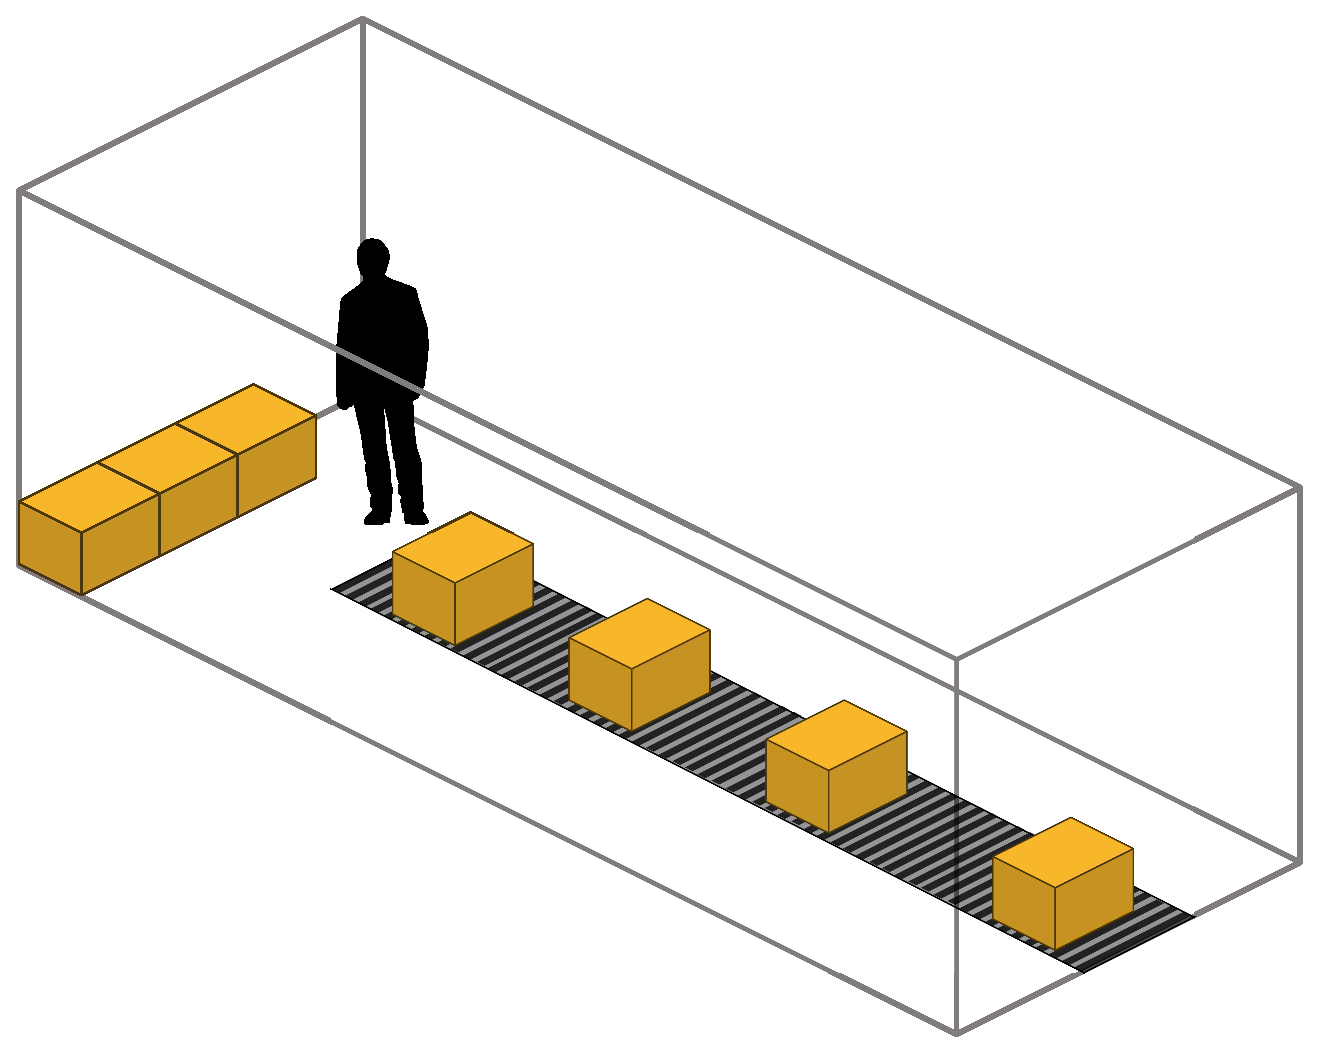
\includegraphics[width=0.5\textwidth]{Figures/cinta_transportadora.eps}
    \caption{Ejemplo del uso de una cinta transportadora.}
    \label{fig:cinta_transportadora}
\end{figure}

La empresa ha implementado un procedimiento específico para guiar a los operadores en la colocación de paquetes dentro del contenedor, con el objetivo de cumplir con todas las condiciones preestablecidas. No obstante, este procedimiento aún no está optimizado y no garantiza la disposición óptima de los paquetes, lo que conduce a una carga subóptima y al desperdicio de espacio.

El desafío que se enfrenta es conocer con anticipación la cantidad de paquetes por tipo que deben cargarse en el contenedor, así como definir el orden de carga y la rotación de cada tipo de paquete. El objetivo es lograr una disposición que no solo cumpla con las restricciones de espacio y los requerimientos del llenado manual, sino que también maximice el valor económico de la carga transportada y la eficiencia en el uso del espacio .

\subsection{Definición formal del problema}

El problema de la carga manual de paquetes en un contenedor se define formalmente de la siguiente manera:

\begin{figure}[H]
    \centering
    \includesvg[width=0.5\textwidth]{Figures/container.svg}
    \caption{Contenedor con dimensiones $W$, $L$, $H$}
    \label{fig:container}
\end{figure}

Siendo un contenedor una caja de forma rectangular, de ancho $W$, largo $L$, alto $H$, en la figura \ref{fig:container} se muestra un contenedor con sus dimensiones, y una capacidad de carga $P$, se tiene definido unos tipos de paquetes también de formas rectangulares $t \in T = \{0, 1, 2, \ldots, n\}$, donde cada tipo $t$ posee ciertas dimensiones de ancho $w_t$, largo $l_t$, alto $h_t$, también posee un peso $p_t$ y un valor $v_t$, además se conoce la cantidad máxima $q^{max}_t$ de paquetes que dispone la empresa por cada tipo.

En este problema, consideramos que $W$, $L$, $H$ y $P$ , $w_t$, $l_t$, $h_t$, $p_t$, $q^{max}_t$ son enteros positivos, los cuales podrían ser representados en unidades de medida centímetros, milímetros, kilogramos, litros, entre otros.

\begin{figure}[H]
    \centering
    \includesvg[width=0.5\textwidth]{Figures/rotacion.svg}
    \caption{Rotación de un paquete en el eje $x$}
    \label{fig:rotation}
\end{figure}

Se tienen restricciones de rotación debido al enfoque de carga manual, en el cual se establece que $\forall r \in r_t, r \in \{0, 1\}, t \in T$ donde $0$ representa que el tipo no se encuentra girado y $1$ que el tipo está girado 90 grados en el eje $x$, esto se puede ver en la figura \ref{fig:rotation} a) sin rotación y b) con rotación. Esto implica que los anchos y largos pueden intercambiarse, mientras que la altura no puede ser modificada.

Por otro lado para facilitar la carga manual, se debe disponer de un orden de carga $o_t$ para cada tipo $t$, donde $o_t \in O = \{0, 1, 2, \ldots, n\}$, que indica el orden en el que se debe cargar cada tipo de paquete en el contenedor.

El problema consiste en determinar la cantidad de paquetes por cada tipo a cargar $\tilde{q}_t$ (la cual se encuentra en torno a la cantidad máxima por tipo, $0 \leq \tilde{q}_t \leq q^{max}_t$) y el orden de carga de cada tipo $o_t$ con determinada rotación $r_t$, de tal modo que se pueda obtener la disposición óptima de los paquetes en el contenedor, asegurando el cumplimiento de las restricciones relacionadas al espacio disponible. Además, se busca maximizar en primer lugar el costo total de la carga ($\max \sum_{t \in T} v_t \cdot \tilde{q}_t$) y en segundo lugar maximizar la utilización del espacio del contenedor ($\max \sum_{t \in T} w_t \cdot l_t \cdot h_t \cdot \tilde{q}_t$).


\subsection{Procedimiento de carga manual}

Para estandarizar la carga manual y facilitar el modelado por ordenador, así como simplificar la labor del operador, se han establecido una serie de supuestos, restricciones y normas que deben seguirse para optimizar la carga de paquetes en el contenedor.

En relación con la definición del problema, se establecen las siguientes suposiciones acerca de los paquetes:

\begin{itemize}
    \item Los paquetes son cajas de forma rectangular.
    \item Los paquetes pueden variar en tamaño, peso y valor.
    \item Los paquetes presentan tamaños y pesos razonables para ser cargados manualmente.
    \item Los paquetes que comparten el mismo tamaño, peso y valor estrictamente se consideran del mismo tipo.
    \item Dos paquetes pueden tener el mismo tamaño y peso pero distinto valor, lo que los convierte en tipos diferentes.
    \item El valor de un paquete no depende de su tamaño o peso, es decir que un paquete sea más grande y pesado que otro no implica que sea de mayor valor y viceversa.
    \item Los paquetes llegan al contenedor agrupados por tipo y en un orden específico.
    \item Los paquetes pueden apilarse unos sobre otros, independientemente de su tipo, pero se debe asegurar la estabilidad de la carga.
    \item Cada tipo de paquete tiene una cantidad fija deseada que debe ser cargada en el contenedor.
    \item Todos los paquetes de un mismo tipo deben mantener la misma orientación.
    \item Los grupos de paquetes llegan en bloques del mismo tipo o de forma secuencial, por ejemplo, a través de cintas transportadoras.
\end{itemize}

Las suposiciones relacionadas con el operario son las siguientes:

\begin{itemize}
    \item Uno o varios operarios realizan la carga de los paquetes en el contenedor de forma manual.
    \item El operario recibe indicaciones previas sobre cómo cargar los paquetes en el contenedor, incluyendo el orden, la cantidad y la orientación de cada tipo de paquete.
    \item Las indicaciones también podrían especificar los espacios que deberán quedar vacíos en el contenedor, los cuales pueden ser llenados con material de relleno para evitar que los paquetes se muevan durante el transporte.
    \item Las indicaciones previas proporcionadas al operario son el resultado de la solución del problema de optimización de la carga.
    \item El objetivo del operario es seguir las indicaciones previas de manera eficiente y precisa, sin necesidad de tomar decisiones adicionales sobre la disposición de los paquetes.
\end{itemize}

El procedimiento de carga manual se basa en la combinación de las suposiciones, restricciones y reglas mencionadas anteriormente, con el objetivo de lograr una carga eficiente y organizada de los paquetes en el contenedor. Este procedimiento se implementa siguiendo una metodología específica que guía al operario en la colocación de los paquetes, asegurando que se cumplan todas las condiciones establecidas.

En el siguiente capítulo se presentará un algoritmo metaheurístico para resolver el problema de optimización de la carga manual de paquetes en un contenedor, considerando las restricciones de espacio del contenedor, así como las restricciones de rotación y orientación de los paquetes.


\newpage
\section{Metaheurística}

\subsection{Codificación de soluciones}
\label{sec:codificacion}

Existen diferentes maneras de codificar las soluciones para el problema de llenado de contenedores. Algunos de los más interesantes son por ejemplo Bortfeldt y otros \cite{GEHRING1997401} que propusieron una codificación basada dobles o simplemente dos listas de igual longitud, la primera representa la secuencia de llenado de los paquetes y la segunda indica la rotación de cada paquete. De manera similar Xianbo y otros [2] propusieron el uso de la primera lista como la secuencia de llenado de cada tipo de paquete y la segunda como la rotación de cada tipo de paquete.

Sin embargo, para las restricciones en nuestro problema, esta codificaciones no son adecuadas ya que necesitamos considerar que las cantidades de un tipo de paquete no son fijas sino que pueden variar de un rango mínimo a un máximo. Por lo tanto, proponemos una codificación basada en 3 listas de igual longitud, la primera lista representa la secuencia de llenado de cada tipo de paquete, la segunda lista indica la rotación de cada tipo de paquete y la tercera lista indica la cantidad de paquetes de cada tipo que se llenan en el contenedor.


Por ejemplo, si tenemos 4 tipos de paquetes $T=\{1,2,3,4\}$, todos los tipos con un mínimo de 0 paquetes y el tipo 1 con un máximo de 10 paquetes $q_1 \in [0,10]$, el tipo 2 con un máximo de 30 paquetes $q_1 \in [0,30]$, el tipo 3 con un máximo de 20 paquetes $q_1 \in [0,20]$ y el tipo 4 con un máximo de 22 paquetes $q_4 \in [0,22]$, una solución factible para el problema de llenado de contenedores podría ser la siguiente:

\begin{figure}[H]
    \centering
    \includesvg[width=0.4\linewidth]{Figures/codificacion.svg}
    \caption{Codificación de una solución con 4 tipos de cajas}
    \label{fig:codificación}
\end{figure}

La primera lista indica que el tipo 2 se llena primero, luego el tipo 1 seguido del tipo 4, y finalmente el tipo 3. La segunda lista indica que el tipo 2 no se rota, el tipo 1 se rota, el tipo 4 se rota y el tipo 3 no se rota. La tercera lista indica que se llenan 27 paquetes del tipo 2, 10 paquetes del tipo 1, 18 paquetes del tipo 4 y 13 paquetes del tipo 3. En la Figura 2 se muestran dos ejemplos adicionales sobre cómo se usa la codificación propuesta para representar soluciones para el problema.

Las tres listas mencionadas son fundamentales para el algoritmo de llenado descrito en la sección 2. Este algoritmo llena el contenedor de manera determinista, siguiendo estrictamente las restricciones establecidas por el problema. Específicamente, una lista determinada siempre resulta en un único método de llenado del contenedor. Si, después de llenar el contenedor, quedan paquetes sobrantes, se procederá a descartar aquellos que no caben, lo que requiere una actualización o corrección de la lista de cantidades de cada tipo de paquete. Este proceso asegura la factibilidad de la solución.

Otra ventaja de esta codificación es la flexibilidad que ofrece para adaptar el problema a diferentes restricciones, por ejemplo si se desea considerar una cantidad fija de paquetes de un tipo, simplemente se puede fijar el mínimo y el máximo de ese tipo de paquete. De igual manera, la estructura soporta si se desea considerar otros tipos de rotaciones, además de las consideradas en el presente trabajo.

Este tipo de codificación permite representar soluciones factibles para el problema de llenado de contenedores, ya que considera la cantidad de paquetes de cada tipo que se llenan en el contenedor. Además, esta codificación es fácil de implementar y de entender, lo que facilita la implementación del algoritmo de llenado y del algoritmo de optimización para resolver el problema.

\subsection{Función de evaluación}

La función de evaluación es una parte fundamental de cualquier algoritmo de optimización, ya que permite evaluar la calidad de las soluciones generadas por el algoritmo. Para el problema de llenado de contenedores, la función de evaluación se puede definir como la suma de los valores de los paquetes que se llenan en el contenedor, es decir, se busca maximizar el valor total de la carga que se llena en el contenedor.

Un paso previo importante antes de calcular el valor total de la carga es verificar si la solución generada es factible, es decir, si al agregar todas las cajas en los ordenes y las posiciones indicadas en la solución, se cumple que todas son colocadas en el contenedor sin superar su capacidad. Para ello, se propone un algoritmo que simula el procedimiento de llenado manual, el cual verifica si una solución generada es factible y si no lo es, lo corrige para que sea factible.

\subsubsection{Algoritmo de llenado manual}

El algoritmo de llenado propuesto está basado en el método Deepest Bottom Left with Fill (DBLF) propuesto por Karabulut y otros \cite{karabulut2004hybrid}, cuyo uso se ha extendido y varios autores han realizado propuestas para mejorarlo o adaptarlo a determinados contextos por ejemplo Wang y otros \cite{wang2010hybrid}, Kang y otros. \cite{kang2012hybrid}. El algoritmo propuesto en el presente trabajo está enfocado en cumplir las restricciones y adaptarse al contexto de un llenado manual de paquetes en un contenedor.

La idea básica del algoritmo DBLF es que los paquetes comienzan a ser llenados en el contenedor de forma secuencial, se prioriza que el paquete se coloque en las siguientes posiciones:

\begin{itemize}
    \item La posición más profunda del contenedor, que ayuda a llenar primero los espacios más alejados de la puerta y evitar obstaculizar el ingreso del operador humano al contenedor.
    \item La posición más baja del contenedor, se da naturalmente debido al efecto de la gravedad, un paquete no podría ser colocado en una posición alta si no se ha llenado primero las posiciones más bajas.
    \item La posición más a la izquierda del contenedor, aunque no es una restricción fuerte, podría usarse el criterio de priorizar la posición más a la derecha si se considera necesario, lo crucial es mantener la consistencia al elegir una de estas dos direcciones. Para el caso de este trabajo se ha elegido la posición más a la izquierda.
\end{itemize}

Al inicio del procedimiento un paquete se coloca en la posición más profunda, más baja y más a la izquierda del contenedor vacío, luego al colocar el paquete en el contenedor, el espacio restante se divide en tres nuevos subespacios, la parte superior, la parte lateral y la parte frontal, en la figura \ref{fig:subespacios} se muestra de cómo se divide el espacio restante en el contenedor al colocar un paquete.

\begin{figure}[H]
    \centering
    \includesvg[width=0.9\textwidth]{Figures/subespacios.svg}
    \caption{División del espacio restante en el contenedor al colocar un paquete. a) Subespacio frontal, b) Subespacio lateral, c) Subespacio superior.}
    \label{fig:subespacios}
\end{figure}

Cada subespacio es considerado como un nuevo contenedor y se repite el proceso de colocar el siguiente paquete en uno de los subespacios creados. Para elegir el siguiente subespacio donde colocar el siguiente paquete, se usa el mismo criterio de priorización DBL, es decir, se elige el subespacio más profundo, más bajo y más a la izquierda, luego se coloca el paquete en dicho subespacio y se repite el proceso.

En la figura \ref{fig:segundo_paquete} se muestra un ejemplo de cómo se coloca un segundo paquete en el contenedor siguiendo el algoritmo DBLF.

\begin{figure}[H]
    \centering
    \includesvg[width=0.5\textwidth]{Figures/segundo_paquete.svg}
    \caption{Ejemplo de colocación de un segundo paquete en el contenedor luego de elegir el último subespacio lateral.}
    \label{fig:segundo_paquete}
\end{figure}

Para este segundo paquete, se ha elegido el anterior subespacio lateral, el cual fué el subespacio más profundo, más bajo y más a la izquierda, siguiendo el criterio de priorización DBL, luego se coloca el paquete en dicho subespacio y se repite el proceso de dividir el espacio restante. Como resultado de esta subdivisión, se obtienen en este caso solamente dos subespacios, la parte superior y la parte lateral, ya que no queda espacio frontal para dividir. En la figura \ref{fig:segundos_subespacios} se muestra estos dos nuevos subespacios.

\begin{figure}[H]
    \centering
    \includesvg[width=0.75\textwidth]{Figures/segundos_subespacios.svg}
    \caption{División del espacio restante en el contenedor al colocar un segundo paquete. a) Nuevo subespacio lateral, b) Nuevo subespacio superior.}
    \label{fig:segundos_subespacios}
\end{figure}

Este procedimiento se repite hasta que se hayan colocado todos los paquetes en el contenedor o no se pueda colocar más paquetes debido a restricciones de espacio. En la figura \ref{fig:contruccion_muro} se muestra como este procedimiento se asemeja a un tipo de construcción de un muro el cuál es otro método de llenado de contenedores.

\begin{figure}[H]
    \centering
    \includesvg[width=0.5\textwidth]{Figures/contruccion_muro.svg}
    \caption{Ejemplo de colocación de más paquetes en el contenedor}
    \label{fig:contruccion_muro}
\end{figure}

El Algoritmo \ref{alg:dblf} muestra el procedimiento de llenado manual de paquetes en un contenedor basado en el algoritmo DBLF.

\begin{algorithm}[H]
    \caption{Algoritmo de llenado manual de paquetes en un contenedor}
    \label{alg:dblf}
    \begin{algorithmic}[1]
        \State $Paquetes \gets \text{lista de paquetes ordenados por tamaño}$
        \State \textbf{Inicialización:} $dblf \gets \text{lista inicializada con el espacio total del contenedor}$
        \State $Contenedor \gets \text{lista vacía para almacenar los paquetes colocados}$
        \For{$paquete \in Paquetes$}
        \State $SubespacioOptimo \gets \text{buscar el subespacio más adecuado en } dblf$
        \If{$SubespacioOptimo \neq \text{null}$}
        \State $Contenedor.\text{add}( \text{colocar}(paquete, SubespacioOptimo) )$
        \State $NuevosSubespacios \gets \text{dividir}(SubespacioOptimo, paquete)$
        \State $dblf.\text{remove}(SubespacioOptimo)$
        \State $dblf.\text{extend}(NuevosSubespacios)$
        \Else
        \State \textbf{print} $\text{"No se encontró espacio para el paquete."}$
        \EndIf
        \EndFor
        \State \Return $Contenedor$
    \end{algorithmic}
\end{algorithm}

El el Algoritmo \ref{alg:dblf}, en la línea 1: se inicializa una lista llamada $Paquetes$ que contiene los paquetes ordenados. Este orden será determinado previamente por el algoritmo de optimización genético, el cual se detallará en la próxima sección. En la línea 2: Se inicializa una lista llamada $dblf$, que representa los subespacios libres en el $Contenedor$. Inicialmente, esta lista contiene un único subespacio que es el contenedor entero. En la línea 3: Se crea una lista vacía llamada $Contenedor$ donde se almacenarán la posición y tamaños de los paquetes que se vayan colocando. Para la parte del proceso de llenado, en la líneas 4: El ciclo for recorre cada paquete en la lista de paquetes.
En la línea 5: Se busca en $dblf$ el primer subespacio disponible que sea suficientemente grande para el paquete. La búsqueda tiene en cuenta que el subespacio debe ser el más profundo, más bajo y más a la izquierda posible donde el paquete pueda caber. En la línea 6: Si tiene una condicional por si se encuentra o no un subespacio adecuado. De continuar con el procedimiento En la línea 7: La función $colocar$ ubica el $paquete$ en la posición más profunda, más baja y más a la izquierda del $SubespacioOptimo$ y devuelve la posición del paquete en el $Contenedor$, la función $add$ agrega el valor devuelto a la lista $Contenedor$. En la línea 8: El subespacio original $SubespacioOptimo$ donde se colocó el paquete se divide hasta en tres nuevos subespacios menores usando la función $dividir$. En la línea 9: se elimina el subespacio original $SubespacioOptimo$ de $dblf$ y en la línea 10: se agregan los nuevos subespacios a la lista $dblf$. En la línea 12: Si no se encuentra un subespacio adecuado para el paquete, se imprime un mensaje de error. Finalmente, en la línea 15: se retorna la lista $Contenedor$ con los paquetes colocados.

En el contexto del llenado manual de contenedores, la propuesta de algoritmo presentado no es suficiente ya que no considera las restricciones propias de un llenado manual, por ejemplo un paquete más grande podría ser colocado encima de varios paquetes más pequeños. Por lo tanto se proponen adaptaciones al algoritmo DBLF para adaptarlo a las restricciones de un llenado manual de contenedores.

\subsubsection{Unión de subespacios}

El primer cambio a considerar es la posibilidad que un paquete pueda ser colocado encima de otros paquetes, en el algoritmo DBLF presentado, un paquete no podía ser colocado encima de otro paquete debido a que los subespacios superiores están separados, por lo tanto se propone una estrategia de unión de subespacios similares. Por ejemplo en la figura \ref{fig:union_subespacios} se muestra como se unen dos subespacios superiores para permitir que un paquete de otro tipo pueda ser colocado encima de otros paquetes.

\begin{figure}[H]
    \centering
    \includesvg[width=0.5\textwidth]{Figures/union_subespacios.svg}
    \caption{Ejemplo de unión de dos subespacios superiores para permitir que un paquete pueda ser colocado encima de otros paquetes.}
    \label{fig:union_subespacios}
\end{figure}

Para realizar la unión de subespacios superiores, se propone un algoritmo de unión de subespacios que se detalla en el Algoritmo \ref{alg:union_subespacios}. Este algoritmo recibe como entrada la lista de subespacios disponibles y recorre dicha lista de atrás hacia adelante, buscando subespacios contiguos y similares para unirlos en un solo subespacio. El algoritmo se detiene cuando no se encuentran más subespacios para unir.

\begin{algorithm}[H]
    \caption{Algoritmo de unión de subespacios}
    \label{alg:union_subespacios}
    \begin{algorithmic}[1]
        \State $Subespacios \gets \text{lista de subespacios disponibles}$
        \State $i \gets \text{longitud de } Subespacios - 1$
        \While{$i > 0$}
        \If{$Subespacios[i].\text{esSimilar}(Subespacios[i-1])$}
        \State $Subespacios[i-1].\text{unir}(Subespacios[i])$
        \State $Subespacios.\text{remove}(Subespacios[i])$
        \EndIf
        \State $i \gets i - 1$
        \EndWhile
        \State \Return $Subespacios$
    \end{algorithmic}
\end{algorithm}

En el Algoritmo \ref{alg:union_subespacios}, en la línea 1: se inicializa una lista llamada $Subespacios$ que contiene los subespacios disponibles en el contenedor. En la línea 2: se inicializa una variable $i$ con la longitud de la lista de subespacios menos uno, esto para iterar siempre el último con el anterior. En la línea 3: Se inicia un ciclo while que recorre la lista de subespacios desde el último hasta el primero. En la línea 4: Se verifica si el subespacio actual y el subespacio anterior son similares, es decir si comparten ciertas características de posición en el contenedor y tamaño. En la línea 5: Si los subespacios son similares, se unen en un solo subespacio y se elimina el subespacio actual de la lista. En la línea 6: Se decrementa el valor de $i$ en uno. En la línea 8: Se retorna la lista de subespacios actualizada.

\subsubsection{Eliminación de subespacios inaccesibles}

En el contexto del llenado manual un espacio se vuelve inaccesible cuando un operador no puede colocar un paquete en dicho espacio debido a que fue bloqueado por otro paquete, en la figura \ref{fig:subespacio_inaccesible} se muestra un ejemplo de un subespacio inaccesible.

\begin{figure}[H]
    \centering
    \includesvg[width=0.5\textwidth]{Figures/subespacio_inaccesible.svg}
    \caption{Ejemplo de un subespacio inaccesible.}
    \label{fig:subespacio_inaccesible}
\end{figure}

La figura \ref{fig:subespacio_inaccesible} muestra desde una perspectiva superior del contenedor, en a) espacios libres en rojo que ha sido bloqueado por un paquete verde colocado, en b) este espacio inaccesible no podrá ser utilizado en su totalidad y se partirá para que quede solo la parte accesible.

Para evitar que un subespacio inaccesible sea considerado en el proceso de llenado, se propone un algoritmo de eliminación de subespacios inaccesibles que se detalla en el Algoritmo \ref{alg:eliminacion_subespacios}. Este algoritmo recibe como entrada la lista de subespacios disponibles y recorre dicha lista desde el último hacia el primero, eliminando o recortando los subespacios inaccesibles.

\begin{algorithm}[H]
    \caption{Algoritmo de eliminación de subespacios inaccesibles}
    \label{alg:eliminacion_subespacios}
    \begin{algorithmic}[1]
        \State $Subespacios \gets \text{lista de subespacios disponibles}$
        \State $i \gets \text{longitud de } Subespacios - 1$
        \While{$i > 0$}
        \If{$Subespacios[i].\text{esInaccesibleParcialmente}()$}
        \State $Subespacios[i].\text{recortar}()$
        \ElsIf{$Subespacios[i].\text{esInaccesibleTotalmente}()$}
        \State $Subespacios.\text{remove}(Subespacios[i])$
        \EndIf
        \State $i \gets i - 1$
        \EndWhile
        \State \Return $Subespacios$
    \end{algorithmic}
\end{algorithm}

En el Algoritmo \ref{alg:eliminacion_subespacios}, en la línea 1: se inicializa una lista llamada $Subespacios$ que contiene los subespacios disponibles en el contenedor. En la línea 2: se inicializa una variable $i$ con la longitud de la lista de subespacios menos uno, esto para iterar siempre desde el último ya que la lista podría ser modificada durante la ejecución del bucle. En la línea 3: Se inicia un ciclo while que recorre la lista de subespacios desde el último hasta el primero. En la línea 4: Se verifica si el subespacio actual es inaccesible parcialmente, es decir si un paquete bloquea parcialmente el subespacio. En la línea 5: Si el subespacio es inaccesible parcialmente, se recorta el subespacio para eliminar la parte inaccesible. En la línea 6: Se verifica si el subespacio actual es inaccesible totalmente, es decir si un paquete bloquea completamente el subespacio. En la línea 7: Si el subespacio es inaccesible totalmente, se elimina el subespacio de la lista. En la línea 8: Se decrementa el valor de $i$ en uno. En la línea 10: Se retorna la lista de subespacios actualizada.

\subsubsection{Eliminación de subespacios profundos}

Un espacio profundo se considera inaccesible cuando un operador no puede alcanzar dicho espacio usando sus brazos, en este caso la distancia máxima que una persona puede alcanzar con sus brazos es una constante a definir en el sistema ya que podría usarse un valor promedio que no resulte en un esfuerzo excesivo para el operador humano. Una estrategia para evitar que un espacio profundo sea considerado en el proceso de llenado es recortar la parte posterior del espacio, en la figura \ref{fig:subespacio_profundo} se muestra un ejemplo de un subespacio profundo.

\begin{figure}[H]
    \centering
    \includesvg[width=0.85\textwidth]{Figures/subespacio_profundo.svg}
    \caption{Ejemplo de un subespacio profundo.}
    \label{fig:subespacio_profundo}
\end{figure}

La figura \ref{fig:subespacio_profundo} muestra desde una perspectiva lateral del contenedor, en a) un espacio profundo en rojo, en b) este espacio profundo ha sido recortado para solo ser considerado la parte frontal accesible.

Para evitar que un subespacio profundo sea considerado en el proceso de llenado, se propone un algoritmo que se detalla en el Algoritmo \ref{alg:eliminacion_subespacios_profundos}. Este algoritmo recibe como entrada la posición de la caja más cercana a la puerta del contenedor para calcular la posición máxima que un operador puede alcanzar con sus manos, y también recibe la lista de subespacios disponibles, recorre dicha lista desde el último hacia el primero, eliminando o recortando los subespacios profundos.

\begin{algorithm}[H]
    \caption{Algoritmo de eliminación de subespacios profundos}
    \label{alg:eliminacion_subespacios_profundos}
    \begin{algorithmic}[1]
        \State $Subespacios \gets \text{lista de subespacios disponibles}$
        \State $PosicionCajaMasCercana \gets \text{posición de la caja más cercana a la puerta}$
        \State $PosicionMaxima \gets \text{posición máxima que un operador puede alcanzar}$
        \State $i \gets \text{longitud de } Subespacios - 1$
        \While{$i > 0$}
        \If{$Subespacios[i].\text{esProfundoParcialmente}(PosicionMaxima)$}
        \State $Subespacios[i].\text{recortar}()$
        \ElsIf{$Subespacios[i].\text{esProfundoTotalmente}(PosicionMaxima)$}
        \State $Subespacios.\text{remove}(Subespacios[i])$
        \EndIf
        \State $i \gets i - 1$
        \EndWhile
        \State \Return $Subespacios$
    \end{algorithmic}
\end{algorithm}

En el Algoritmo \ref{alg:eliminacion_subespacios_profundos}, en la línea 1: se inicializa una lista llamada $Subespacios$ que contiene los subespacios disponibles en el contenedor. En la línea 2: se inicializa una variable $PosicionCajaMasCercana$ con la posición de la caja más cercana a la puerta del contenedor contando el largo de la caja, el cuál daría el punto más cercano a la puerta del contenedor. En la línea 3: se inicializa una variable $PosicionMaxima$ con la posición máxima que un operador puede alcanzar con sus brazos, se calcula usando el punto más cercano a la puerta del contenedor menos la distancia establecida que los brazos de un operador puede alcanzar. En la línea 4: se inicializa una variable $i$ con la longitud de la lista de subespacios menos uno, esto para iterar siempre desde el último ya que la lista podría ser modificada durante la ejecución del bucle. En la línea 5: Se inicia un ciclo while que recorre la lista de subespacios desde el último hasta el primero. En la línea 6: Se verifica si el subespacio actual es profundo parcialmente. En la línea 7: Si el subespacio es profundo parcialmente, se recorta el subespacio para eliminar la parte profunda y se mantiene la parte más frontal accesible. En la línea 8: Se verifica si el subespacio actual es profundo totalmente. En la línea 9: Si el subespacio es profundo totalmente, se elimina el subespacio completamente de la lista. En la línea 10: Se decrementa el valor de $i$ en uno. En la línea 12: Se retorna la lista de subespacios actualizada.

\subsubsection{Algoritmo de llenado manual adaptado}

El Algoritmo \ref{alg:dblf_adaptado} muestra el procedimiento de llenado manual de paquetes en un contenedor considerando que los paquetes se reciben por tipos además usando las estrategias de unión de subespacios, eliminación de subespacios inaccesibles y eliminación de subespacios profundos.

\begin{algorithm}[H]
    \caption{Algoritmo de llenado manual de paquetes en un contenedor adaptado}
    \label{alg:dblf_adaptado}
    \begin{algorithmic}[1]
        \State \textbf{Parámetros:} $Tipos \gets \text{lista de tipos de paquetes}$
        \State \textbf{Inicialización:} $dblf \gets \text{lista inicializada con el espacio total del contenedor}$
        \State $Contenedor \gets \text{lista vacía para almacenar los paquetes colocados}$
        \For{$tipo \in Tipos$}
        \For{$i \gets 1 \text{ to } tipo.cantidad$}
        \State $SubespacioOptimo \gets \text{buscar el subespacio más adecuado en } dblf$
        \If{$SubespacioOptimo \neq \text{null}$}
        \State $Contenedor.\text{add}( \text{colocar}(tipo, SubespacioOptimo) )$
        \State $NuevosSubespacios \gets \text{dividir}(SubespacioOptimo, tipo)$
        \State $dblf.\text{remove}(SubespacioOptimo)$
        \State $dblf.\text{extend}(NuevosSubespacios)$
        \Else
        \State \textbf{print} $\text{"No se encontró espacio para el paquete."}$
        \EndIf
        \EndFor
        \State $dblf \gets \text{unirSubespacios}(dblf)$
        \State $dblf \gets \text{eliminarSubespaciosInaccesibles}(dblf)$
        \State $dblf \gets \text{eliminarSubespaciosProfundos}(dblf)$
        \EndFor
        \State \Return $Contenedor$
    \end{algorithmic}
\end{algorithm}

En el Algoritmo \ref{alg:dblf_adaptado}, en la línea 1: se recibe una lista llamada $Tipos$ que contiene los tipos de paquetes cuya información incluye el tamaño, rotación y cantidad de paquetes. En la línea 2: Se inicializa una lista llamada $dblf$, que representa los subespacios libres en el $Contenedor$. Inicialmente, esta lista contiene un único subespacio que es el contenedor entero. En la línea 3: Se crea una lista vacía llamada $Contenedor$ donde se almacenarán la posición y tamaños de los paquetes que se vayan colocando. Para la parte del proceso de llenado, en la línea 4: El ciclo for recorre cada tipo de paquete en la lista de tipos. En la línea 5: Se inicia un ciclo for que recorre la cantidad de paquetes por tipo. En la línea 6: Se busca en $dblf$ el primer subespacio disponible que sea suficientemente grande para el paquete. La búsqueda tiene en cuenta que el subespacio debe ser el más profundo, más bajo y más a la izquierda posible donde el paquete pueda caber. En la línea 7: Si tiene una condicional por si se encuentra o no un subespacio adecuado. De continuar con el procedimiento En la línea 8: La función $colocar$ ubica el $tipo$ en la posición más profunda, más baja y más a la izquierda del $SubespacioOptimo$ y devuelve la posición del paquete en el $Contenedor$, la función $add$ agrega el valor devuelto a la lista $Contenedor$. En la línea 9: El subespacio original $SubespacioOptimo$ donde se colocó el paquete se divide hasta en tres nuevos subespacios menores usando la función $dividir$. En la línea 10: se elimina el subespacio original $SubespacioOptimo$ de $dblf$ y en la línea 11: se agregan los nuevos subespacios a la lista $dblf$. En la línea 16: Se unen los subespacios similares en $dblf$ usando la función $unirSubespacios$. En la línea 17: Se eliminan los subespacios inaccesibles en $dblf$ usando la función $eliminarSubespaciosInaccesibles$. En la línea 18: Se eliminan los subespacios profundos en $dblf$ usando la función $eliminarSubespaciosProfundos$. En la línea 20: Se retorna la lista $Contenedor$ con los paquetes colocados.

\subsubsection{Mejora adicional al algoritmo de llenado}

Debido a la naturaleza altamente aleatoria propias de un algoritmo genético, es posible que se generen soluciones que se encuentren muy próximas de ser muy buenas pero que no evaluaron los espacios locales de manera adecuada, por lo que se propone un ajuste al algoritmo de llenado manual para que pueda aumentar la cantidad de cajas cuando sea posible de tal modo que se pueda aprovechar al máximo el espacio disponible.


\begin{figure}[H]
    \centering
    \includesvg[width=0.5\textwidth]{Figures/llenado_adicional.svg}
    \caption{Ejemplo de llenado adicional de un paquete tipo T1 donde ya se ha llenado dos tipos T1 (7 Cajas) y T2 (2 Cajas).}
    \label{fig:llenado_adicional}
\end{figure}

Por ejemplo, en la Figura \ref{fig:llenado_adicional} se ilustra un caso donde se ha completado el llenado de un tipo T1 específico con 7 paquetes y un tipo T2 con 2 paquetes, pero aún queda un espacio no usado donde podría ser aprovechado para añadir un octavo paquete del mismo tipo T1, siempre y cuando aún dispongamos de paquetes adicionales de ese tipo.

Esta situación presenta dos posibles mejoras para la gestión de paquetes. La primera consiste en añadir un paquete justo después de completar la carga de paquetes del mismo tipo. Esta opción podría optimizar el uso del espacio disponible de forma más eficiente, aunque existe el riesgo de que pueda deteriorar la calidad de la solución, ya que podría inferir en la colocación de los siguientes tipos de cajas. La segunda mejora propuesta es añadir el paquete una vez que se hayan llenado completamente todos los paquetes de todos los tipos. Si bien esta estrategia asegura que la calidad de la solución no se vea comprometida, podría no siempre haber muchos espacios libres que puedan ser aprovechados.

La primera mejora es llamada \textit{llenado adicional inmediato} y denominada M1, y la segunda mejora es llamada \textit{llenado adicional al final} y denominada  M2. Ambas mejoras solo se pueden aplicar en circunstancias específicas durante la ejecución del algoritmo genético y su rendimiento será evaluado en la sección de experimentos.

A continuación se resume el algoritmo de llenado manual adaptado con las mejoras M1 en el Algoritmo \ref{alg:dblf_adaptado_mejoras_m1}.

\begin{algorithm}[H]
    \caption{Algoritmo de llenado manual de paquetes en un contenedor adaptado con la mejora M1}
    \label{alg:dblf_adaptado_mejoras_m1}
    \begin{algorithmic}[1]
        \State \textbf{Parámetros:} $Tipos \gets \text{lista de tipos de paquetes}$
        \State \textbf{Inicialización:} $dblf \gets \text{lista inicializada con el espacio total del contenedor}$
        \State $Contenedor \gets \text{lista vacía para almacenar los paquetes colocados}$
        \For{$tipo \in Tipos$}
        \For{$i \gets 1 \text{ to } tipo.cantidad$}
        \State \text{...} \Comment{Mismo procedimiento que en el Algoritmo \ref{alg:dblf_adaptado}}
        \If{$i = tipo.cantidad$}
        \State $dblfSuperior \gets \text{filtrar solo subespacios superiores en } dblf$
        \State $SubespacioLibre \gets \text{buscar el subespacio más adecuado en } dblfSuperior$
        \If{$SubespacioLibre \neq \text{null}$}
        \State $tipo.cantidad \gets tipo.cantidad + 1$
        \EndIf
        \EndIf
        \EndFor
        \State \text{...} \Comment{Mismo procedimiento que en el Algoritmo \ref{alg:dblf_adaptado}}
        \EndFor
        \State \Return $Contenedor$
    \end{algorithmic}
\end{algorithm}

El Algoritmo \ref{alg:dblf_adaptado_mejoras_m1} es similar al Algoritmo \ref{alg:dblf_adaptado} con la diferencia de que se añade un paquete adicional del mismo tipo justo después de completar la carga de paquetes del mismo tipo. En la línea 7: Se verifica si el paquete actual es el último paquete del tipo, si es así, en la línea 8: se filtran solo los subespacios superiores en $dblf$ y en la línea 9: se busca el subespacio más adecuado en $dblfSuperior$. En la línea 10: Si se encuentra un subespacio adecuado, en la línea 11: se incrementa la cantidad de paquetes del tipo en uno, esto para que el bucle no termina hasta que se haya colocado el paquete adicional. En las siguientes líneas se realiza el mismo procedimiento que en el Algoritmo \ref{alg:dblf_adaptado}. En la línea 17: Se retorna la lista $Contenedor$ con los paquetes colocados.

Para el caso de la mejora M2 se sigue un procedimiento distinto, ya que se añade un paquete adicional una vez que se han llenado completamente todos los paquetes de todos los tipos. A continuación se resume el algoritmo de llenado manual adaptado con la mejora M2 en el Algoritmo \ref{alg:dblf_adaptado_mejoras_m2}.

\begin{algorithm}[H]
    \caption{Algoritmo de llenado manual de paquetes en un contenedor adaptado con la mejora M2}
    \label{alg:dblf_adaptado_mejoras_m2}
    \begin{algorithmic}[1]
        \State \textbf{Parámetros:} $Tipos \gets \text{lista de tipos de paquetes}$
        \State \textbf{Inicialización:} $dblf \gets \text{lista inicializada con el espacio total del contenedor}$
        \State $Contenedor \gets \text{lista vacía para almacenar los paquetes colocados}$
        \State $EspaciosSobrantes \gets \text{lista vacía para almacenar los espacios sobrantes}$
        \For{$tipo \in Tipos$}
        \For{$i \gets 1 \text{ to } tipo.cantidad$}
        \State \text{...} \Comment{Mismo procedimiento que en el Algoritmo \ref{alg:dblf_adaptado}}
        \EndFor
        \If{$existeEspacioSobrante(dblf)$}
        \State $EspaciosSobrantes \gets \text{filtrar solo subespacios sobrantes en } dblf$
        \EndIf
        \EndFor
        \State \text{...}
        \For{$tipo \in Tipos$}
        \For{$i \gets tipo.cantidad \text{ to } tipo.cantidadMaxima$}
        \State $SubespacioLibre \gets \text{buscar el subespacio más adecuado en } EspaciosSobrantes$
        \If{$SubespacioLibre \neq \text{null}$}
        \State $Contenedor.\text{add}( \text{colocar}(tipo, SubespacioLibre) )$
        \State $tipo.cantidad \gets tipo.cantidad + 1$
        \EndIf
        \EndFor
        \EndFor
        \State \text{...} \Comment{Mismo procedimiento que en el Algoritmo \ref{alg:dblf_adaptado}}
        \State \Return $Contenedor$
    \end{algorithmic}
\end{algorithm}

El Algoritmo \ref{alg:dblf_adaptado_mejoras_m2} también es similar al Algoritmo \ref{alg:dblf_adaptado} con la diferencia de que se durante todo el procedimiento de llenado se van recopilando los espacios libres para que luego se añada un paquete adicional una vez que se han llenado completamente todos los paquetes de todos los tipos. En la línea 9: Se verifica si existe algún espacio sobrante en $dblf$, si es así, en la línea 10: se filtran solo los subespacios sobrantes en $dblf$ y se almacenan en $EspaciosSobrantes$. En las siguientes líneas se realiza el mismo procedimiento que en el Algoritmo \ref{alg:dblf_adaptado}. En la línea 14: Se recorre nuevamente la lista de tipos de paquetes y en la línea 15: se recorre la cantidad de paquetes que faltan por añadir. En la línea 16: Se busca el subespacio más adecuado en $EspaciosSobrantes$. En la línea 17: Si se encuentra un subespacio adecuado, en la línea 18: se añade el paquete al contenedor y en la línea 19: se actualiza la cantidad de paquetes del tipo. En las siguientes líneas se realiza el mismo procedimiento que en el Algoritmo \ref{alg:dblf_adaptado}. En la línea 24: Se retorna la lista $Contenedor$ con los paquetes colocados.

Como se ha podido observar en los algoritmos presentados, si bien ambos tipos de mejoras tienen la misma finalidad de añadir paquetes adicionales al contenedor, cada una tiene sus propias ventajas y desventajas, por lo que se propone evaluar el rendimiento de cada una de ellas en la sección de experimentos.


\subsection{Población inicial}

Para generar la población inicial se propone un mecanismo simple de generación de soluciones aleatorias. Dado un conjunto de tipos de paquetes $T = \{1,2, \ldots, n\}$, donde cada tipo de paquete $t_i \in T$ tiene un mínimo y un máximo de paquetes a insertar en el contenedor $t_i \in [t_i^{min},t_i^{max}]$, se generan soluciones aleatorias de la siguiente manera:

\begin{enumerate}
    \item Se selecciona aleatoriamente un tipo de paquete $t_i \in T$.
    \item Se selecciona aleatoriamente un tipo de rotación $r_i \in R, R \in \{0,1\}$.
    \item Se selecciona aleatoriamente una cantidad de paquetes $q_i \in [t_i^{min},t_i^{max}]$.
    \item Se repiten los pasos 1 al 3 hasta que se hayan seleccionado todos los tipos de paquetes.
    \item Se repiten los pasos 1 al 4 hasta que se hayan generado $N$ soluciones.
\end{enumerate}

El algoritmo de generación de la población inicial se muestra en el Algoritmo~\ref{alg:generacionPoblacionInicial}. En este algoritmo, $T$ es el conjunto de tipos de paquetes, $R$ es el conjunto de rotaciones, $N$ es el tamaño de la población, $t_i^{min}$ y $t_i^{max}$ son el mínimo y el máximo de paquetes de cada tipo, respectivamente, y $P$ es la población inicial.

\begin{algorithm}[H]
    \caption{Generación de la población inicial}\label{alg:generacionPoblacionInicial}
    \begin{algorithmic}[1]
        \Require $T, R, N$
        \Ensure $P$
        \State $P \leftarrow \emptyset$
        \For{$i = 1$ to $N$}
        \State $S \leftarrow \emptyset$
        \For{each $t_i \in T$}
        \State $r \leftarrow$ rotación aleatoria de $R$
        \State $q \leftarrow$ cantidad aleatoria de paquetes entre $t_i^{\min}$ y $t_i^{\max}$
        \State $S \leftarrow S \cup \{(t_i, r, q)\}$
        \EndFor
        \State $P \leftarrow P \cup \{S\}$
        \EndFor
        \State \Return $P$
    \end{algorithmic}
\end{algorithm}

En el Algoritmo~\ref{alg:generacionPoblacionInicial}, en la línea 1: se inicializa una lista vacía $P$ que contendrá la población inicial. En el ciclo for de la línea 2: se itera para generar $N$ soluciones. En la línea 3: se inicializa una lista vacía $S$ que representa una solución. En el ciclo for de la línea 4: se itera para seleccionar aleatoriamente un tipo de paquete del conjunto de tipos $T$. En las línea 5: se selecciona aleatoriamente una rotación del conjunto de rotaciones $R$. En la línea 6: se selecciona aleatoriamente una cantidad de paquetes de acuerdo al mínimo y máximo de paquetes de cada tipo. En la línea 7: se añade el tipo de paquete, la rotación y la cantidad de paquetes a la solución $S$. En la línea 9: se añade la solución a la población. En la línea 11: se retorna la población generada.

De esta manera, las soluciones aleatorias generadas respetan las restricciones específicas del problema. Esto asegura que la cantidad de cada tipo de paquete insertado en el contenedor cumple con los rangos establecidos, manteniéndose entre el mínimo y el máximo definidos. Adicionalmente, se establece que estas cantidades sean generadas como números enteros, manteniendo la integridad de las soluciones conforme a las necesidades del problema.

\subsection{Selección}

Para seleccionar las soluciones que se utilizarán en cada generación del algoritmo evolutivo, se propone un mecanismo de selección basado en el método de torneo usando un tamaño de torneo de 2, también conocido como torneo binario. Anand y otros [3] lo describen como uno de los más eficientes métodos de selección para algoritmos evolutivos. Para usar el método de torneo binario, se seleccionan aleatoriamente dos soluciones de la población y se selecciona la mejor solución de las dos. Este proceso se lleva a cabo junto con el operador de cruce para lo cual cada padre se selecciona mediante un torneo binario.

En el Algoritmo~\ref{alg:seleccionPadres}, $P$ es la población, $N$ es el tamaño de la población, $P1$ y $P2$ son los padres seleccionados.

\begin{algorithm}[H]
    \caption{Selección de padres}\label{alg:seleccionPadres}
    \begin{algorithmic}[1]
        \Require $P, N$
        \Ensure $P1, P2$
        \State $P1 \leftarrow \emptyset$
        \State $P2 \leftarrow \emptyset$
        \For{$i = 1$ to $N$}
        \State $S1, S2 \leftarrow$ soluciones aleatorias de $P$
        \If{$S1$ > $P1$}
        \State $P1 \leftarrow P1 \cup S1$
        \Else
        \State $P1 \leftarrow P1 \cup S2$
        \EndIf
        \State $S3, S4 \leftarrow$ soluciones aleatorias de $P$
        \If{$S3$ > $P2$}
        \State $P2 \leftarrow P2 \cup S3$
        \Else
        \State $P2 \leftarrow P2 \cup S4$
        \EndIf
        \EndFor
        \State \Return $P1, P2$
    \end{algorithmic}
\end{algorithm}

En el Algoritmo~\ref{alg:seleccionPadres}, en la línea 1 y 2: se inicializan dos listas vacías $P1$ y $P2$ que contendrán los padres seleccionados. En el ciclo for de la línea 3: se itera para todo el tamaño de la población $N$. En las línea 4: se seleccionan aleatoriamente dos soluciones de la población $P$. En las líneas de la 5 a la 9: se selecciona la mejor solución de las dos y se añade a la lista $P1$. En las líneas de la 10 a la 15: se vuelve a repetir el proceso para seleccionar el segundo padre y se añade a la lista $P2$. En la línea 17: se retornan los padres seleccionados.

De acuerdo a lo anterior, se generan dos listas de padres que se utilizarán en el operador de cruce para generar una nueva población. Este método de selección procura que siempre se tienda a seleccionar soluciones mejores aunque tampoco se descartan soluciones peores, lo que permite mantener la diversidad en la población.

\subsection{Cruce}

Como se vió en la selección de padres, se generaron dos listas $P1$ y $P2$ que se utilizarán en el operador de cruce para generar una nueva población. Para el operador de cruce se propone un mecanismo de cruce basado en el cruce de un punto. Según \textcite{Umbarkar2015}, para este tipo de operador, se selecciona un punto aleatorio en el vector solución y se intercambian las partes de las dos soluciones que están a la izquierda y a la derecha del punto. Este operador de cruce es simple y fácil de implementar, y se ha demostrado que es eficiente para resolver problemas de optimización combinatoria.

Es importante destacar que el operador de cruce se aplica a una fracción específica de la población, determinada por una tasa de cruce, $P_{CROSS}$. Esta tasa representa la probabilidad de que dos soluciones seleccionadas sean cruzadas. La implementación de este mecanismo promueve la diversidad dentro de la población y fomenta la generación de nuevas soluciones potencialmente superiores a las existentes.

En el Algoritmo~\ref{alg:crucePadresGenerico}, $P1$ y $P2$ son los padres seleccionados, $C1$ y $C2$ son los hijos generados, $N$ es el tamaño de la población y $T$ es el conjunto de tipos de paquetes.

\begin{algorithm}[H]
    \caption{Cruce de padres genérico}\label{alg:crucePadresGenerico}
    \begin{algorithmic}[1]
        \Require $P1, P2, N, T$
        \Ensure $C1, C2$

        \State $C1 \leftarrow \emptyset$
        \State $C2 \leftarrow \emptyset$
        \State $p \leftarrow$ punto aleatorio en la solución
        \For{$i = 1$ to $N$}
        \If{$i \leq p$}
        \State $C1 \leftarrow C1 \cup P1[i]$
        \State $C2 \leftarrow C2 \cup P2[i]$
        \Else
        \State $C1 \leftarrow C1 \cup P2[i]$
        \State $C2 \leftarrow C2 \cup P1[i]$
        \EndIf
        \EndFor
        \State \Return $C1, C2$
    \end{algorithmic}
\end{algorithm}

Por lo tanto, al intentar aplicar el algoritmo sobre la Codificación de Soluciones propuesta en la sección \ref{sec:codificacion}, se puede representar en la Figura \ref{fig:cruce_simple} el cruce de dos padres $P1$ y $P2$.

\begin{figure}[H]
    \centering
    \includesvg[width=0.5\textwidth]{Figures/cruce_simple.svg}
    \caption{Cruce de dos padres $P1$ y $P2$}
    \label{fig:cruce_simple}
\end{figure}

Como puede verse en la Figura \ref{fig:cruce_simple}, se selecciona un punto aleatorio en la solución (en este caso se encuentra en la quinta posición) y si se intercambian las partes de las dos soluciones que están a la izquierda y a la derecha del punto, las soluciones hijas resultantes tendrían una alta probabilidad de ser no factibles ya que se estarían repitiendo tipos de paquetes en el contenedor.

Si bien este algoritmo de cruce es ampliamente aplicable a diversos tipos de problemas, es particularmente adaptable al problema de llenado de contenedores, teniendo en cuenta la codificación propuesta en la sección \ref{sec:codificacion}. Se propone, por tanto, un mecanismo de cruce diseñado para asegurar la factibilidad de las soluciones generadas. Este método consiste en utilizar la primera partición de la solución de un progenitor y completarla con los tipos de paquetes aún no seleccionados de la misma partición. De esta manera, se asegura que cada solución generada, o hijo, contenga todos los tipos de paquetes, garantizando su viabilidad.

En la Figura \ref{fig:cruce_propuesto} se muestra el cruce de dos padres $P1$ y $P2$ utilizando el algoritmo de cruce propuesto.

\begin{figure}[H]
    \centering
    \includesvg[width=0.75\textwidth]{Figures/cruce_propuesto.svg}
    \caption{Cruce de dos padres $P1$ y $P2$ utilizando el algoritmo de cruce propuesto}
    \label{fig:cruce_propuesto}
\end{figure}

Como se ilustra en la Figura \ref{fig:cruce_propuesto}, el proceso de cruce se detalla para los padres P2 y P1. A P2 le faltan los tipos de paquetes T3, T5 y T7; tras buscar en P1, se agregan en el orden encontrado: T5, T7, T3. En el caso de P1, le faltan los tipos T1, T6 y T3, que al buscarse en P2 se encuentran y se añaden en el orden de T6, T1 y T3. Este método asegura que las soluciones generadas, C1 y C2, sean factibles al completar los tipos de paquetes faltantes en cada padre, manteniendo así la viabilidad de las soluciones.

Por lo tanto, el algoritmo propuesto, adaptado a la codificación, para el cruce de padres se muestra en el Algoritmo~\ref{alg:crucePadresPropuesto}.

\begin{algorithm}[H]
    \caption{Cruce de padres propuesto}\label{alg:crucePadresPropuesto}
    \begin{algorithmic}[1]
        \Require $P1, P2, N, T$
        \Ensure $C1, C2$

        \State $C1 \leftarrow \emptyset$
        \State $C2 \leftarrow \emptyset$
        \State $p \leftarrow$ punto aleatorio en la solución
        \For{$i = 1$ to $N$}
        \If{$i \leq p$}
        \State $C1 \leftarrow C1 \cup P1[i]$
        \State $C2 \leftarrow C2 \cup P2[i]$
        \Else
        \For{each $t_i \in T$}
        \If{$C1$ no contiene $P2[i]$}
        \State $C1 \leftarrow C1 \cup P2[i]$
        \EndIf
        \If{$C2$ no contiene $P1[i]$}
        \State $C2 \leftarrow C2 \cup P1[i]$
        \EndIf
        \EndFor
        \EndIf
        \EndFor
        \State \Return $C1, C2$
    \end{algorithmic}
\end{algorithm}

En el Algoritmo~\ref{alg:crucePadresPropuesto}, en las líneas 1 y 2 se inicializan dos listas vacías $C1$ y $C2$ que contendrán los hijos generados. En la línea 3 se selecciona un punto aleatorio $p$ en la solución de tamaño $N$. En el ciclo for de la línea 4 se itera para todo el tamaño de la población $N$. En las líneas de la 5 a la 8 se conservan las primeras $p$ posiciones de los padres $P1$ y $P2$ respectivamente. En la línea 9 se inicia un ciclo para cada tipo de paquete $t_i \in T$. En las líneas de la 10 a la 12 se verifica si el hijo $C1$ no contiene el tipo de paquete $P2[i]$ y si es así se añade a $C1$. En las líneas de la 13 a la 15 se verifica si el hijo $C2$ no contiene el tipo de paquete $P1[i]$ y si es así se añade a $C2$. En la línea 19 se retorna los dos hijos generados $C1$ y $C2$.

Consecuentemente, se asegura que las soluciones generadas no solo sean factibles y abarquen todos los tipos de paquetes, sino que también difieran de las soluciones padres, contribuyendo así a la preservación de la diversidad dentro de la población.

\subsection{Mutación}

Según \textcite{Dockhorn2022}, la mutación consiste en aplicar pequeños cambios a las soluciones candidatas para tratar de explorar nuevas regiones locales del espacio de búsqueda. Para el presente problema, ya que codificación propuesta consta de tres listas, se propone también tres operadores de mutación, uno para cada lista. El primer tipo de mutación intercambia dos tipos de paquetes en la secuencia de llenado junto a su rotación y cantidad específica, el segundo tipo de mutación solo intercambia la rotación de un tipo de paquete y el tercer tipo de mutación cambia la cantidad de paquetes de un tipo de paquete.

Cabe mencionar que el operador de mutación se aplica a una proporción muy pequeña de la población, dependiendo de una tasa de mutación $P_{MUT}$, que se define como la probabilidad de que una solución seleccionada mute y generé una nueva solución cercana a la inicial.

En la Figura \ref{fig:mutacion_tipo} se muestra un ejemplo de mutación de un tipo de paquete en la secuencia de llenado, se elige dos tipos de paquetes aleatorios y se intercambian.

\begin{figure}[H]
    \centering
    \includesvg[width=0.5\textwidth]{Figures/mutacion_tipos.svg}
    \caption{Mutación de un tipo de paquete en la secuencia de llenado}
    \label{fig:mutacion_tipo}
\end{figure}

En la Figura \ref{fig:mutacion_rotacion} se muestra un ejemplo de mutación de la rotación de un tipo de paquete en la secuencia de llenado, se elige un tipo de paquete aleatorio y se cambia la rotación del estado 0 (no rotado) hacia el estado 1 (rotado).

\begin{figure}[H]
    \centering
    \includesvg[width=0.5\textwidth]{Figures/mutacion_rotacion.svg}
    \caption{Mutación de la rotación de un tipo de paquete en la secuencia de llenado}
    \label{fig:mutacion_rotacion}
\end{figure}

En la Figura \ref{fig:mutacion_cantidad} se muestra un ejemplo de mutación de la cantidad de paquetes de un tipo de paquete en la secuencia de llenado, se elige un tipo de paquete aleatorio y se cambia la cantidad de paquetes.

\begin{figure}[H]
    \centering
    \includesvg[width=0.5\textwidth]{Figures/mutacion_cantidad.svg}
    \caption{Mutación de la cantidad de paquetes de un tipo de paquete en la secuencia de llenado}
    \label{fig:mutacion_cantidad}
\end{figure}

Aunque estos tres tipos de mutación no se pueden aplicar a la vez, se puede seleccionar el tipo de mutación aleatoriamente y aplicarla a la solución seleccionada. Por lo tanto, el algoritmo de mutación se muestra en el Algoritmo~\ref{alg:mutacion}. En este algoritmo, $S$ es la solución a mutar, $T$ es el conjunto de tipos de paquetes, $R$ es el conjunto de rotaciones, $t_i^{\min}$ y $t_i^{\max}$ son el mínimo y el máximo de paquetes de cada tipo, respectivamente, y $S'$ es la solución mutada.

\begin{algorithm}[H]
    \caption{Mutación de soluciones}\label{alg:mutacion}
    \begin{algorithmic}[1]
        \Require $S, T, R, t_i^{\min}, t_i^{\max}$
        \Ensure $S'$
        \State $S' \leftarrow S$
        \State $m \leftarrow$ número aleatorio entre 1 y 3
        \If{$m = 1$}
        \State $i, j \leftarrow$ dos números aleatorios entre 1 y $|T|$
        \State $S'[i], S'[j] \leftarrow S[j], S[i]$
        \ElsIf{$m = 2$}
        \State $i \leftarrow$ número aleatorio entre 1 y $|T|$
        \State $S'[i] \leftarrow$ intercambio de rotación de $S[i]$
        \ElsIf{$m = 3$}
        \State $i \leftarrow$ número aleatorio entre 1 y $|T|$
        \State $q \leftarrow$ variar la cantidad paquetes de $S[i]$
        \State $S'[i] \leftarrow q$
        \EndIf
        \State \Return $S'$
    \end{algorithmic}
\end{algorithm}

En el Algoritmo~\ref{alg:mutacion}, en la línea 1 se inicializa una solución mutada $S'$ con la solución original $S$. En la línea 2 se selecciona aleatoriamente un número $m$ entre 1 y 3 que representa el tipo de mutación a aplicar. En la línea 3 se verifica si el número aleatorio es igual a 1, si es así, en las líneas 4 y 5 se seleccionan dos números aleatorios $i$ y $j$ entre 1 y el tamaño de $T$ y se intercambian los tipos de paquetes en las posiciones $i$ y $j$ de la solución $S'$. En la línea 6 se verifica si el número aleatorio es igual a 2, si es así, en la línea 7 se selecciona un número aleatorio $i$ entre 1 y el tamaño de $T$ y en la linea 8 se intercambia la rotación del tipo de paquete en la posición $i$ de la solución $S'$. En la línea 9 se verifica si el número aleatorio es igual a 3, si es así, en las líneas 10 se selecciona un número aleatorio $i$ entre 1 y el tamaño de $T$. En la línea 11 se varía la cantidad de paquetes del tipo de paquete en la posición $i$ de la solución $S'$, esto implica que la cantidad puede incrementar o disminuir. En la línea 14 se retorna la solución mutada $S'$.

\subsection{Elitismo}

Según \textcite{Hasni2013}, el principio del elitismo consiste en mantener las mejores soluciones de una generación a la siguiente, lo que permite garantizar que siempre se mantenga la mejor solución encontrada hasta el momento, ya que los operadores de cruce y mutación pueden generar soluciones las cuales no sean mejores que las soluciones actuales, en dicho caso se reemplazan el mejor individuo de la generación anterior por el peor individuo de la generación actual.

Por lo tanto, se propone un mecanismo de elitismo que garantice que siempre se mantenga la mejor solución encontrada hasta el momento. Para ello, se selecciona la mejor solución de la población actual y se compara con la mejor solución élite encontrada hasta el momento. Si la mejor solución de la población actual es mejor que la mejor solución élite encontrada hasta el momento, se sustituye la mejor solución élite por la mejor solución de la población actual, de lo contrario, la solución élite reemplaza a la peor solución de la población actual.

El algoritmo de elitismo se muestra en el Algoritmo~\ref{alg:elitismo}. En este algoritmo, $P$ es la población actual, $S$ es la mejor solución encontrada hasta el momento y $S'$ es la mejor solución de la población actual.

\begin{algorithm}[H]
    \caption{Elitismo}\label{alg:elitismo}
    \begin{algorithmic}[1]
        \Require $P, S$
        \Ensure $S'$
        \State $S' \leftarrow$ mejor solución de $P$
        \If{$S'$ > $S$}
        \State $S \leftarrow S'$
        \Else
        \State $P \leftarrow$ reemplazo de la peor solución de $P$ por $S$
        \EndIf
        \State \Return $S$
    \end{algorithmic}

\end{algorithm}

En el Algoritmo~\ref{alg:elitismo}, en la línea 1 se selecciona la mejor solución de la población actual $P$ y se almacena en $S'$. En la línea 2 se usa la función de evaluación para verificar si la mejor solución de la población actual $S'$ es mejor que la mejor solución encontrada hasta el momento $S$, si es así, en la línea 3 se reemplaza la mejor solución encontrada hasta el momento $S$ por la mejor solución de la población actual $S'$. Si la verificación de la linea 2 es falsa, en la línea 5 se reemplaza la peor solución de la población actual $P$ por la mejor solución encontrada hasta el momento $S$. En la línea 6 se retorna la mejor solución  $S$ que se mantendrá en las generaciones futuras.

Como resultado, se asegura la preservación de la mejor solución identificada hasta el momento, evitando su pérdida en futuras generaciones.

\subsection{Algoritmo genético}

Con todos los operadores definidos, se puede definir el algoritmo genético completo. En el Algoritmo~\ref{alg:algoritmoGenetico}, $T$ es el conjunto de tipos de paquetes, $R$ es el conjunto de rotaciones, $N$ es el tamaño de la población, $P_{CROSS}$ es la tasa de cruce, $P_{MUT}$ es la tasa de mutación y $G$ es la condiciones de parada que podría ser una cantidad máxima de tiempo, una cantidad máxima de generaciones en que la mejor solución no ha mejorado o simplemente una cantidad máxima de generaciones en total.

\begin{algorithm}[H]
    \caption{Algoritmo genético}\label{alg:algoritmoGenetico}
    \begin{algorithmic}[1]
        \Require $T, R, N, P_{CROSS}, P_{MUT}, G$
        \Ensure $S$
        \State $P \leftarrow$ generación de la población inicial
        \State $S \leftarrow$ mejor solución de $P$
        \While {(no se cumpla la condición de parada $G$)}
        \State $P1,P2 \leftarrow$ Realizar selección en $P$
        \State $P \leftarrow$ Realizar cruzamiento en $P1$ y $P2$ con tasa $P_{CROSS}$
        \State $P \leftarrow$ Aplicar mutación a $P$ con tasa $P_{MUT}$
        \State $S \leftarrow$ Realizar elitismo en $P$ con $S$
        \EndWhile
        \State \Return $S$
    \end{algorithmic}
\end{algorithm}

En el Algoritmo~\ref{alg:algoritmoGenetico}, en la línea 1 se genera la población inicial $P$. En la línea 2 se usa la función de evaluación para seleccionar la mejor solución de la población inicial $P$ y se almacena en $S$. En el ciclo while de las líneas 3 a 8 se itera mientras no se cumpla la condición de parada $G$. En las línea 4 se seleccionan los padres $P1$ y $P2$ de la futura generación y en la linea 5 se realiza el cruce de los padres seleccionados con una tasa de cruce $P_{CROSS}$. En la línea 6 se aplica la mutación a la población $P$ (que ya paso por el operador de cruce) con una tasa de mutación $P_{MUT}$. En la línea 7 se realiza el elitismo en la población $P$ (que ya paso por los operadores de cruce y mutación) con la mejor solución élite $S$. En la línea 9 se retorna la mejor solución $S$ encontrada.

Al finalizar el algoritmo, se obtiene la mejor solución encontrada que representa la mejor forma de llenar el contenedor con los paquetes disponibles de modo que se maximice el valor total de los paquetes colocados y que se cumplan las restricciones prácticas del problema.

\newpage
\section{Estudio experimental}

\subsection{Datos de prueba}

\subsection{Diseño del experimento}

\subsection{Resultados y análisis}

\newpage
\section{Conclusiones}

    \lipsum[4]

\newpage
\input{appendix}

\newpage
\input{References}

\end{document}